{
\usebackgroundtemplate{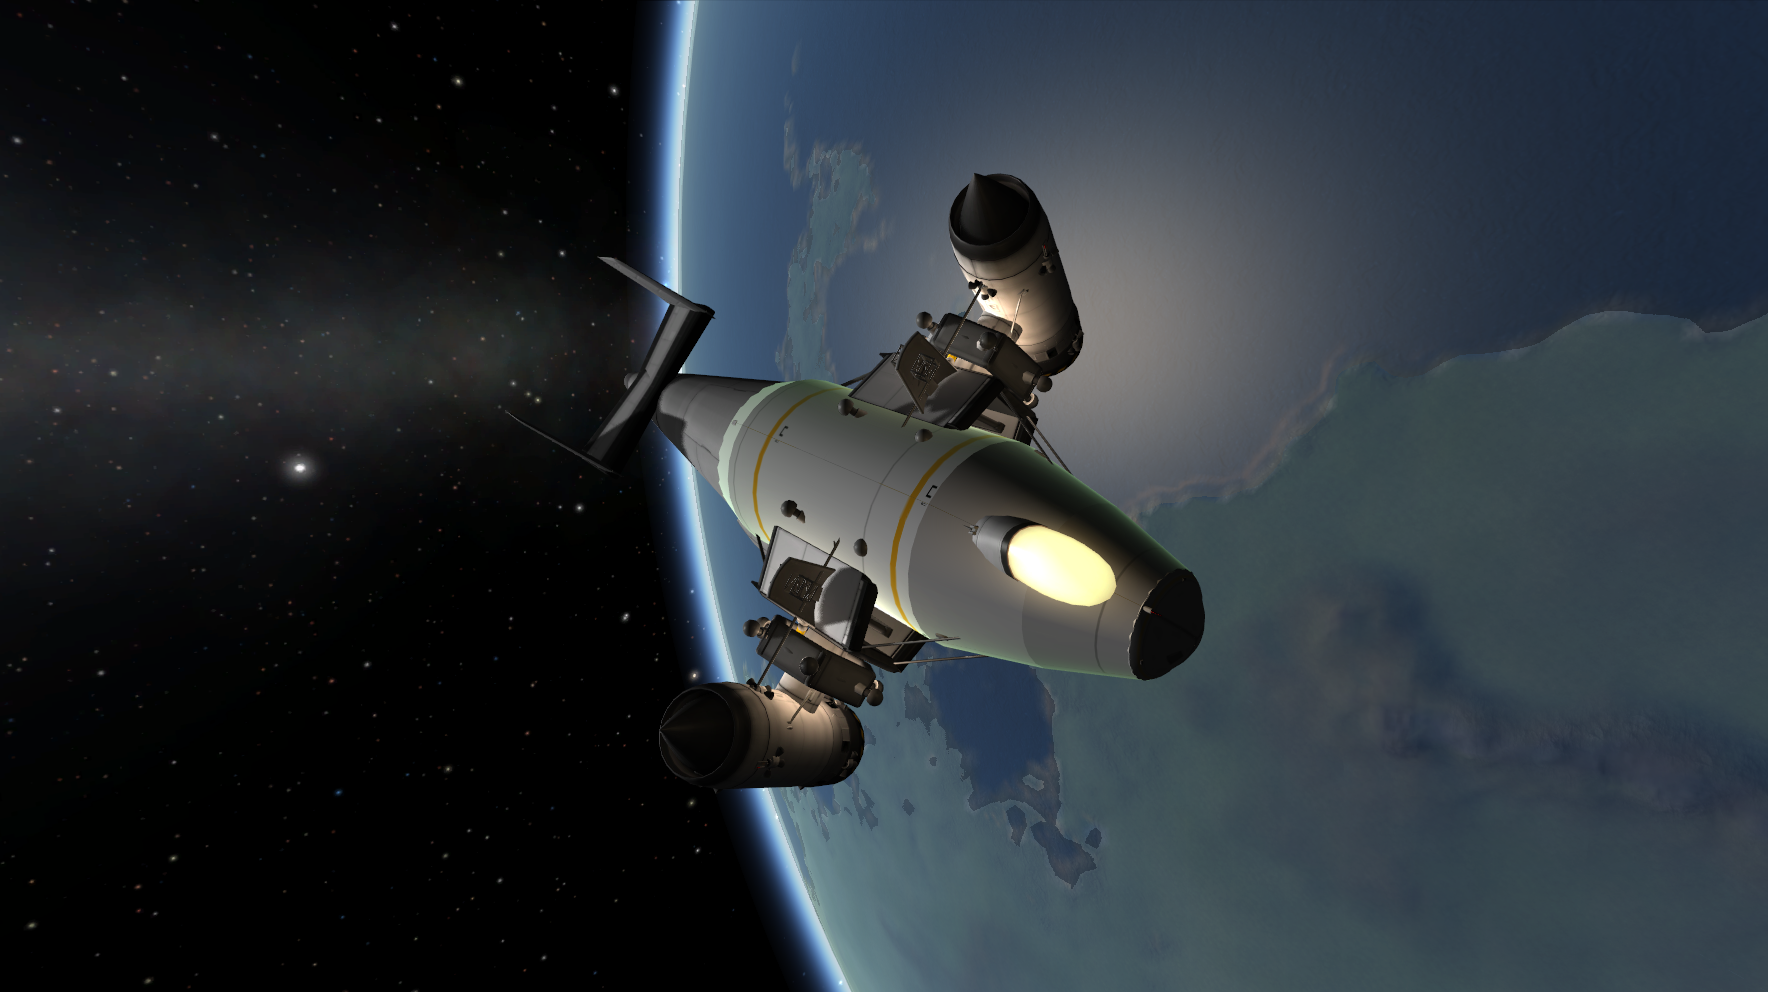
\includegraphics[height=\paperheight,keepaspectratio]{images/intro}}%
\begin{frame}
    \frametitle{Introduction}
    \begin{block}{}
        \begin{itemize}
            \item We'll take you through launching a rocket and landing it on a different planet
            \item Obviously: this is simplified
        \end{itemize}
    \end{block}
\end{frame}
\begin{frame}
    \frametitle{Technicalities}
    \begin{block}{Orbit}
        \begin{itemize}
            \item An object rotating around another object is said to be in orbit
        \end{itemize}
    \end{block}
\end{frame}
\begin{frame}
    \frametitle{Technicalities}
    \begin{block}{Delta-v}
        \begin{itemize}
            \item Your fuel budget
            \item How much can I accelerate/decelerate my rocket
            \item Depends on thrust to weight ratio
        \end{itemize}
    \end{block}
\end{frame}
}
